%%%%%%%%%%%%%%%%%%%%%%%%%%%%%%%%%%%%%%%%%%%%%%%%%%%%%%%%%%%
% --------------------------------------------------------
% Tau
% LaTeX Template
% Version 2.4.4 (28/02/2025)
%
% Author: 
% Guillermo Jimenez (memo.notess1@gmail.com)
% 
% License:
% Creative Commons CC BY 4.0
% --------------------------------------------------------
%%%%%%%%%%%%%%%%%%%%%%%%%%%%%%%%%%%%%%%%%%%%%%%%%%%%%%%%%%%

\documentclass[9pt,a4paper,twocolumn,twoside]{tau-class/tau}
\usepackage[brazil]{babel}

\usepackage{booktabs}
\usepackage{float}
\usepackage{graphicx}
\usepackage{siunitx}

%% Spanish babel recomendation
% \usepackage[spanish,es-nodecimaldot,es-noindentfirst]{babel} 

%% Draft watermark
% \usepackage{draftwatermark}

%----------------------------------------------------------
% TITLE
%----------------------------------------------------------

\journalname{Relatório de Sistemas de Controle I - Etapa 1}
\title{Controle de Estabilização de um Pêndulo Invertido Rotacional}

%----------------------------------------------------------
% AUTHORS, AFFILIATIONS AND PROFESSOR
%----------------------------------------------------------

\author[a,1]{JOSÉ A. DA SILVA}
\author[b,2]{KAUA LESSA L. DOS SANTOS }
\author[c,3]{PABLO MUNIH S. DE CARVALHO}
\author[d,4]{PLÁCIDO AUGUSTUS DE O. CORDEIRO}

%----------------------------------------------------------

\affil[a]{Engenharia da Computação, Universidade Federal de Alagoas}
\affil[b]{Engenharia da Computação, Universidade Federal de Alagoas}
\affil[c]{Engenharia da Computação, Universidade Federal de Alagoas}

\professor{Prof. ICARO BEZERRA QUEIROZ DE ARAUJO}

%----------------------------------------------------------
% FOOTER INFORMATION
%----------------------------------------------------------

\institution{Universidade Federal de Alagoas}
%\footinfo{\LaTeX\ Template}%
\theday{\today}
% \leadauthor{Aluno et al.} %
\course{Engenharia da Computação}

%----------------------------------------------------------
% ABSTRACT AND KEYWORDS
%----------------------------------------------------------

\begin{abstract}    
    Este relatório apresenta a primeira etapa do projeto da disciplina de sistemas de controle 1, de um pêndulo invertido rotacional. Será inicialmente abordado a descrição do sistema, justificativa da relevância, objetivos, materiais necessários e cronograma de execução.
\end{abstract}

%----------------------------------------------------------

\keywords{pêndulo invertido, controle rotacional, estabilização, sistemas não lineares}

%----------------------------------------------------------

\begin{document}
		
    \maketitle 
    \thispagestyle{firststyle} 
    \tauabstract 
    % \tableofcontents
    % \linenumbers 
    
%----------------------------------------------------------

\section{Introdução}
    \taustart{O} pêndulo invertido é um sistema clássico utilizado como plataforma de testes no estudo de controle de sistemas dinâmicos instáveis. 
    Seu comportamento não linear e naturalmente instável o torna ideal para o desenvolvimento e avaliação de diferentes estratégias de controle. 
    Esse tipo de sistema está presente em aplicações reais como segways, foguetes e robôs bípedes autobalanceados.

    \subsection{Importância}

    De acordo com \cite{casas2024}, os modelos de pêndulos são úteis tanto por razões pedagógicas e de pesquisa, como por
    representarem versões simplificadas de sistemas mecânicos que surgem na robótica e sistemas espaciais. Já \cite{breganon2021}
    destaca modelos de pêndulos, como o aeropêndulo e o Pêndulo de Furuta, como ferramentas importantes para o ensino de conteúdos
    relacionados ao controle de sistemas. 

    \subsection{Arquiteturas}

    Na literatura, é possível encontrar duas arquiteturas principais de pêndulos invertidos:
    A linear (Figura~\ref{fig:pendulos}a), considerada a forma mais comum de pêndulo invertido, tem o pêndulo montado sobre uma base com um carrinho
    que pode se movimentar livremente sobre um plano horizontal \cite{diao2016}; E o modelo rotacional (Figura~\ref{fig:pendulos}b), também conhecido
    como Pêndulo de Furuta, onde o pêndulo está conectado a um braço giratório acionado por um motor. Este último representa 
    um sistema subatuado e com maior complexidade dinâmica, sendo mais desafiador do ponto de vista de controle.

    \begin{figure}[H]
    \centering
    \caption{(a) Pêndulo Invertido Linear. (b) Pêndulo Invertido Rotacional.}
    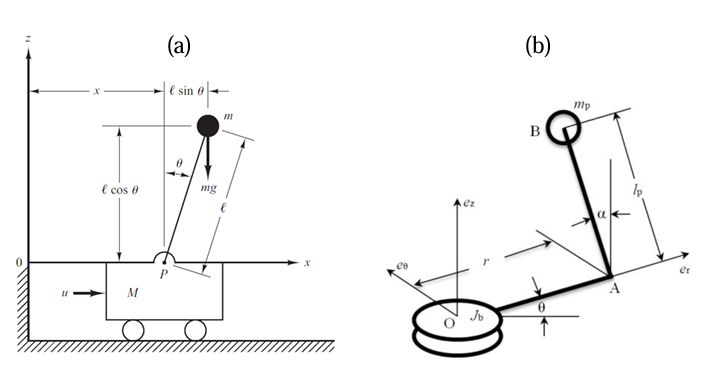
\includegraphics[width=0.8\columnwidth]{figures/pendulos.png} 
    \label{fig:pendulos}
    \caption*{Fonte: \cite{Ogata2010} e \cite{Nath2014}.}
\end{figure}

    O Pêndulo de Furuta foi proposto por Katsuhita Furuta em 1992 no Instituto de Tecnologia de Tóquio \cite{houck2013},
    e tem sido amplamente utilizado em contextos acadêmicos e experimentais. Devido às suas características, o modelo 
    rotacional foi o escolhido neste projeto.

    \subsection{Objetivo}

    Este relatório apresenta a primeira etapa do desenvolvimento de um sistema de controle para estabilização do pêndulo rotacional.
    Os objetivos incluem a descrição conceitual do sistema, definição das variáveis envolvidas, revisão de abordagens de controle
    aplicadas e levantamento dos materiais e métodos necessários para a implementação prática e simulação do protótipo.

\section{Descrição do Sistema}

    O sistema proposto consiste em um \textbf{pêndulo invertido rotacional}, também conhecido como Pêndulo de Furuta. Trata-se de uma estrutura clássica na área de controle de sistemas dinâmicos, composta por uma barra vertical (pêndulo) acoplada a um braço horizontal giratório, que é acionado por um motor DC. A base do sistema permanece fixa, e o movimento ocorre simultaneamente em dois planos: o braço gira no plano horizontal, enquanto o pêndulo oscila no plano vertical.

    Esse tipo de pêndulo é especialmente interessante do ponto de vista didático e experimental, pois combina características desafiadoras como a instabilidade natural e a subatuação — ou seja, o número de entradas de controle (um único motor) é inferior ao número de variáveis dinâmicas relevantes (dois ângulos). Isso impõe restrições significativas ao projeto do controlador, que deve ser capaz de estabilizar o sistema mesmo com essa limitação.

    \subsection{Funcionamento do Sistema}
    
    O motor aplica um torque $\tau$ na base giratória, fazendo com que o braço horizontal, com inércia $I_0$, rotacione ao redor do eixo vertical. Essa rotação transfere momento ao pêndulo, gerando uma interação dinâmica entre os dois corpos. A gravidade atua diretamente sobre o pêndulo vertical, fazendo com que ele tenda naturalmente a cair. O objetivo do sistema de controle é calcular e aplicar um torque adequado no braço giratório para gerar forças inerciais que mantenham o pêndulo em pé, na posição vertical invertida.

    A interação entre os dois graus de liberdade ($\theta_0$ e $\theta_1$) cria um sistema acoplado e não linear. A ausência de controle direto sobre o pêndulo (pois o motor atua apenas sobre o braço) impõe desafios adicionais, exigindo que o controlador manipule o braço de forma inteligente para influenciar o movimento do pêndulo de maneira indireta, especialmente durante oscilações rápidas ou diante de perturbações externas.

    \subsection{Variáveis do Sistema}
    
    O sistema possui uma única entrada e duas saídas principais:
    
    \begin{itemize}
        \item \textbf{Variável de entrada (atuador):} torque $\tau$ aplicado pelo motor na base.
        \item \textbf{Variáveis de saída (controladas):}
        \begin{itemize}
        \item $\theta_0$: ângulo de rotação da base (braço horizontal), medido pelo \textit{encoder acoplado ao motor}. Representa o movimento de rotação no plano horizontal.
        \item $\theta_1$: ângulo do pêndulo em relação à vertical, medido pelo \textit{encoder incremental} localizado no eixo de articulação entre o pêndulo e o braço horizontal. Essa é a principal variável a ser estabilizada pelo controle, idealmente mantendo-se próxima de zero (posição vertical invertida).
        \end{itemize}
    \end{itemize}

    Além dessas variáveis, outros parâmetros físicos são essenciais para a modelagem e controle do sistema, como as massas dos componentes ($m_0$, $m_1$), os comprimentos dos braços ($L_0$, $L_1$), os momentos de inércia ($I_0$, $I_1$) e a constante gravitacional $g$.

    o ponto de vista de modelagem em espaço de estados, o sistema é classificado como um sistema dinâmico não linear de quarta ordem, pois seu comportamento é descrito por quatro variáveis de estado:
    \begin{itemize}
    
    \item $\theta_0$ e sua derivada temporal $\omega_0$ (velocidade angular do braço)

    \item $\theta_1$ e sua derivada temporal $\omega_1$ (velocidade angular do pêndulo).
    
    \end{itemize}
    Essas quatro variáveis constituem o vetor de estado e são suficientes para representar completamente a evolução dinâmica do sistema ao longo do tempo.

    \subsection{Esquema do Sistema}
    
    A Figura~\ref{fig:esquema} apresenta uma representação tridimensional do sistema, destacando os principais parâmetros físicos e as coordenadas angulares relevantes. Esse modelo será utilizado como referência para a modelagem matemática e implementação do controlador nas etapas seguintes do projeto.
    
    \begin{figure}[H]
        \centering
        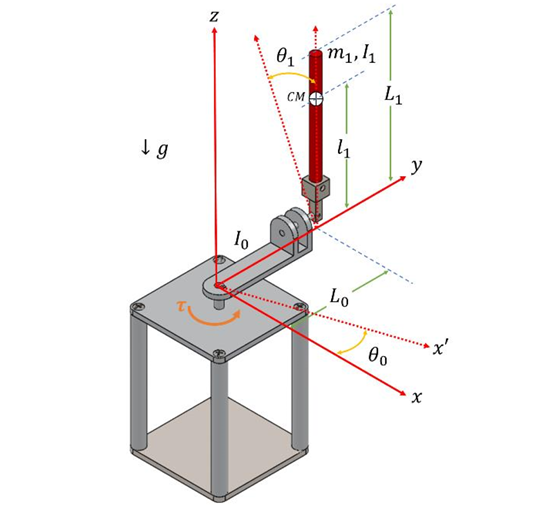
\includegraphics[width=0.85\columnwidth]{figures/pendulo com angulos.png}
        \caption{Representação tridimensional do pêndulo invertido rotacional com seus parâmetros físicos e coordenadas. Fonte: \cite{Duart2017}}
        \label{fig:esquema}
    \end{figure}
   

\section{Revisão Bibliográfica}

   O controle de um pêndulo rotacional invertido normalmente é dividido em duas etapas: swing-up (balanço inicial), que leva o pêndulo da posição para baixo até próximo da posição invertida, e estabilização, que mantém o pêndulo equilibrado no ponto de equilíbrio.

    Diversas estratégias podem ser utilizadas na fase de estabilização. Estudos como os de \cite{mathew2013} mostram que controladores PID bem sintonizados podem apresentar desempenho satisfatório em torno do ponto de equilíbrio, sendo uma boa escolha para projetos introdutórios. Outras técnicas mais avançadas incluem o controle por linearização por realimentação, detalhado na obra de \cite{spong2008}, o controle robusto não linear, exemplificado por \cite{Furuta1992}, e o controle preditivo baseado em modelo (MPC), como abordado por \cite{deepak2019l}, mas estas exigem maior conhecimento em controle.

        Além dessas variáveis, outros parâmetros físicos são essenciais para a modelagem e controle do sistema, como as massas dos componentes ($m_0$, $m_1$), os comprimentos dos braços ($L_0$, $L_1$), os momentos de inércia ($I_0$, $I_1$) e a constante gravitacional $g$.

    Neste trabalho, adotaremos como principal referência o documento elaborado por \cite{yamane2021} intitulado “Projeto Mecânico e Síntese do Controlador de um Pêndulo de Furuta”. Essa obra propõe diretamente a modelagem do pêndulo invertido rotacional

    O autor apresenta uma modelagem detalhada baseada em:
    \begin{itemize}

    \item Cálculo da energia cinética e potencial do sistema
    
    \item Aplicação das equações de Euler-Lagrange  
    
    \item Obtenção das equações de movimento para os subsistemas mecânico e eletromecânico
    
    
    \item Construção de um modelo não linear acoplado no ambiente 
    MATLAB Simulink
    \end{itemize}

    Além disso, o trabalho realiza a síntese e simulação de um controlador LQR, validando os resultados por meio de experimentos com um protótipo real.
    
    Adicionalmente, será utilizada como referência complementar prática a obra “Modular Control of a Rotary Inverted Pendulum System” \cite{diao2016}, que apresenta uma abordagem didática e direta para implementação prática do controle de um pêndulo rotacional. Essa obra fornece os modelos dinâmicos (linear e não linear), parâmetros físicos e estratégias de controle PID e swing-up modulares, sendo ideal para aplicação em ambiente real e simulações no MATLAB/Simulink. Sua linguagem clara e foco na execução o fizeram um bom candidato para esse projeto.


\section{Materiais e Métodos Propostos}

    Para a implementação do sistema, serão utilizados os seguintes componentes, organizados em categorias de componentes eletrônicos e mecânicos.

    \subsection{Componentes Eletrônicos}
    \begin{itemize}
        \item \textbf{Microcontrolador:} Esp32 \cite{esp32Datasheet}, utilizado para controle do sistema de balanceamento e leitura dos sensores.
        \item \textbf{Motor com Encoder:} JGA25-371 12V DC 18-1930RPM \cite{mot4datasheet}, motor DC com encoder incremental para acionar o pêndulo e medir o ângulo.
        \item \textbf{Driver de Motor (Ponte H):} BTS7960 \cite{bts7960datasheet}, utilizado para controlar a direção e a velocidade do motor.
        \item \textbf{Encoder Incremental:} E38S6G5-600B-G24N \cite{e38s6g5datasheet}, para medir a posição do pêndulo e enviar os dados de feedback para o microcontrolador.
        \item \textbf{Fonte de Alimentação:} Fonte de 12V para alimentar os motores, encoder e o microcontrolador.
    \end{itemize}

    \subsection{Componentes Mecânicos}
    \begin{itemize}
        \item \textbf{Estrutura impressa em 3D:} A estrutura do protótipo será totalmente impressa em 3D, incluindo a base e os suportes necessários para o sistema de pêndulo.
        \item \textbf{Parafusos:} Para fixação das partes mecânicas, serão usados parafusos, assegurando que os componentes fiquem firmemente montados.
    \end{itemize}
    
    \begin{figure}[H]
        \centering
        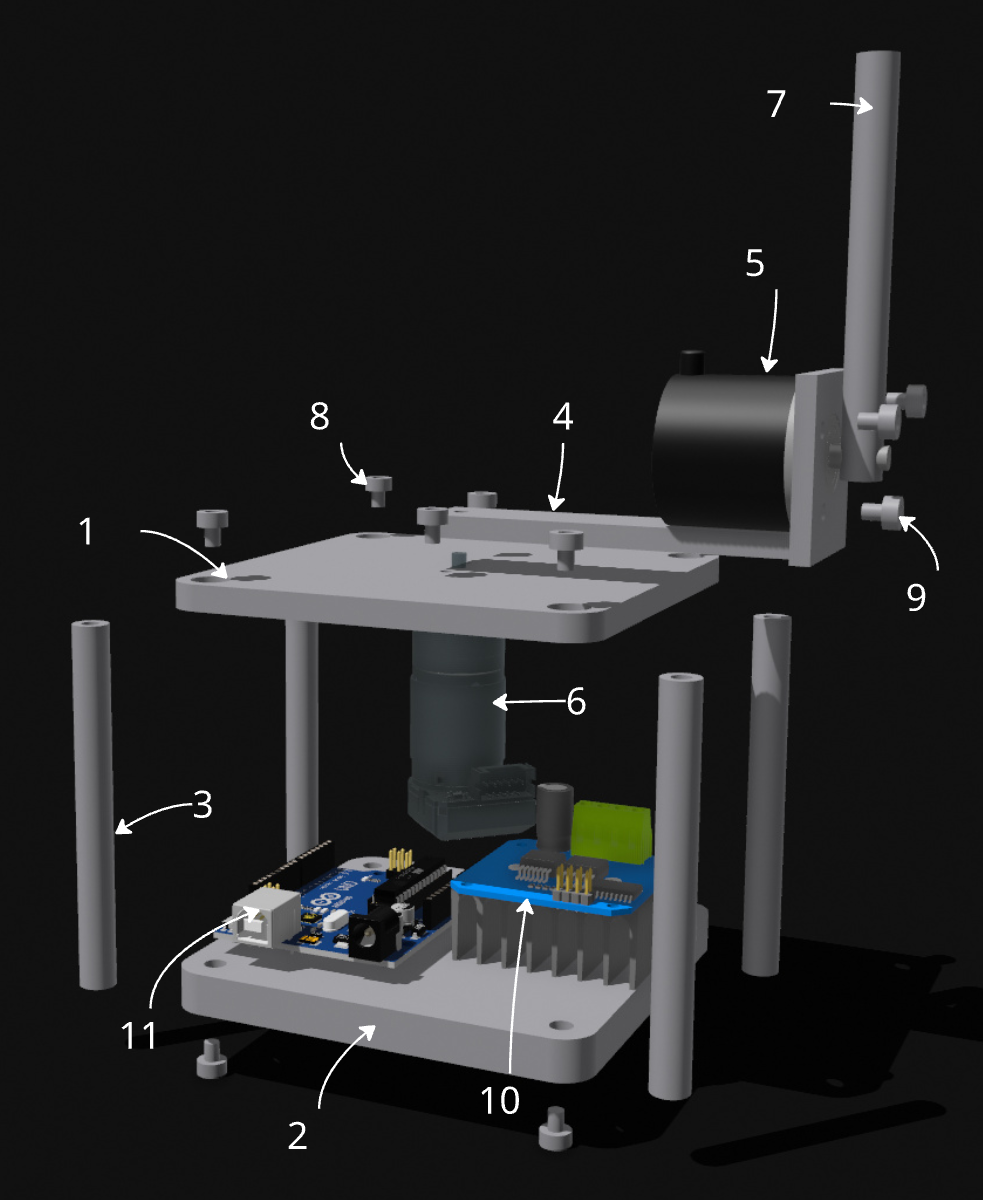
\includegraphics[width=0.8\columnwidth]{figures/itens.png}
        \caption{Esquema do Pêndulo Invertido Rotacional e seus Componentes.}
        \label{fig:itens}
    \end{figure}
    
    \begin{table}[H]
        \centering
        \caption{Lista de Peças Utilizadas na Construção do Protótipo}
        \label{tab:lista_pecas}
        \begin{tabular}{lllll}
            \toprule
            \textbf{Número} & \textbf{Peça} & \textbf{Qtd}  & \textbf{Preço} \\
            \midrule
            1  & Topo                    & 1   & R\$ - \\
            2  & Base                    & 1   & R\$ - \\
            3  & Suporte                 & 4   & R\$ - \\
            4  & Braço                   & 1   & R\$ - \\
            5  & Encoder Incremental     & 1   & R\$ 80,34 \\
            6  & Motor com Encoder       & 1   & R\$ 55,17 \\
            7  & Pêndulo                 & 1   & R\$ - \\
            8  & Parafuso M3x6           & 5   & R\$ 2,00 \\
            9  & Parafuso M6x25          & 8   & R\$ 4,00 \\
            10 & Ponte H                 & 1   & R\$ 31,56 \\
            11 & Esp Wroom 32            & 1   & R\$ 33,04 \\
            Total & -                    & -   & R\$ 206,11 \\
            \bottomrule
        \end{tabular}
        \caption*{Note: A quantidade dos componentes foi estimada com base no modelo 3D e pode ser ajustada durante a montagem.}
    \end{table}
    \vspace{-6mm}
    \subsection{Descrição do Circuito e Ligações}

    O circuito do sistema é composto por um microcontrolador ESP32 DevKit, responsável pelo controle do motor, leitura dos encoders e execução dos algoritmos de estabilização do pêndulo. A Figura~\ref{fig:circuito} ilustra as conexões entre os principais componentes.

    A alimentação principal é fornecida por uma fonte de \SI{12}{\volt}, que alimenta diretamente o driver de motor BTS7960 pelos terminais \texttt{B+} e \texttt{B-}. O mesmo GND da fonte é compartilhado com o GND do ESP32 para garantir a referência comum entre os sinais de controle e potência.

    O motor DC com encoder Hall integrado é conectado ao BTS7960 pelos terminais \texttt{M+} e \texttt{M-}, responsáveis pela potência do motor, e também por quatro fios adicionais que compõem o encoder Hall:
    \begin{itemize}
        \item \textbf{VCC (vermelho)} – Alimentação de \SI{5}{\volt} fornecida pelo pino \texttt{VIN} do ESP32.
        \item \textbf{GND (preto)} – Terra comum ao ESP32 e à fonte.
        \item \textbf{Canal A} – Ligado ao pino \texttt{GPIO34} do ESP32 (entrada apenas), utilizado para leitura de pulsos do encoder.
        \item \textbf{Canal B} – Ligado ao pino \texttt{GPIO35} do ESP32 (entrada apenas), utilizado para determinar o sentido de rotação.
    \end{itemize}

    O pêndulo é instrumentado com um encoder incremental E38S6G5-600B-G24N, que possui saída de dois canais (A e B) em quadratura. Esses sinais são conectados aos pinos \texttt{GPIO32} e \texttt{GPIO33} do ESP32, permitindo a leitura da posição angular e do sentido de movimento.

    O controle de velocidade e direção do motor é realizado via sinais PWM gerados pelo ESP32:
    \begin{itemize}
        \item \textbf{RPWM} – Pino \texttt{GPIO25}, responsável pelo controle de rotação em sentido horário.
        \item \textbf{LPWM} – Pino \texttt{GPIO26}, responsável pelo controle de rotação em sentido anti-horário.
        \item \textbf{EN-R} e \textbf{EN-L} – Pinos \texttt{GPIO27} e \texttt{GPIO14}, respectivamente, usados para habilitar os canais do driver (podendo ser fixados em nível lógico alto se não for necessário controle via software).
    \end{itemize}

    \begin{figure}[H]
        \centering
        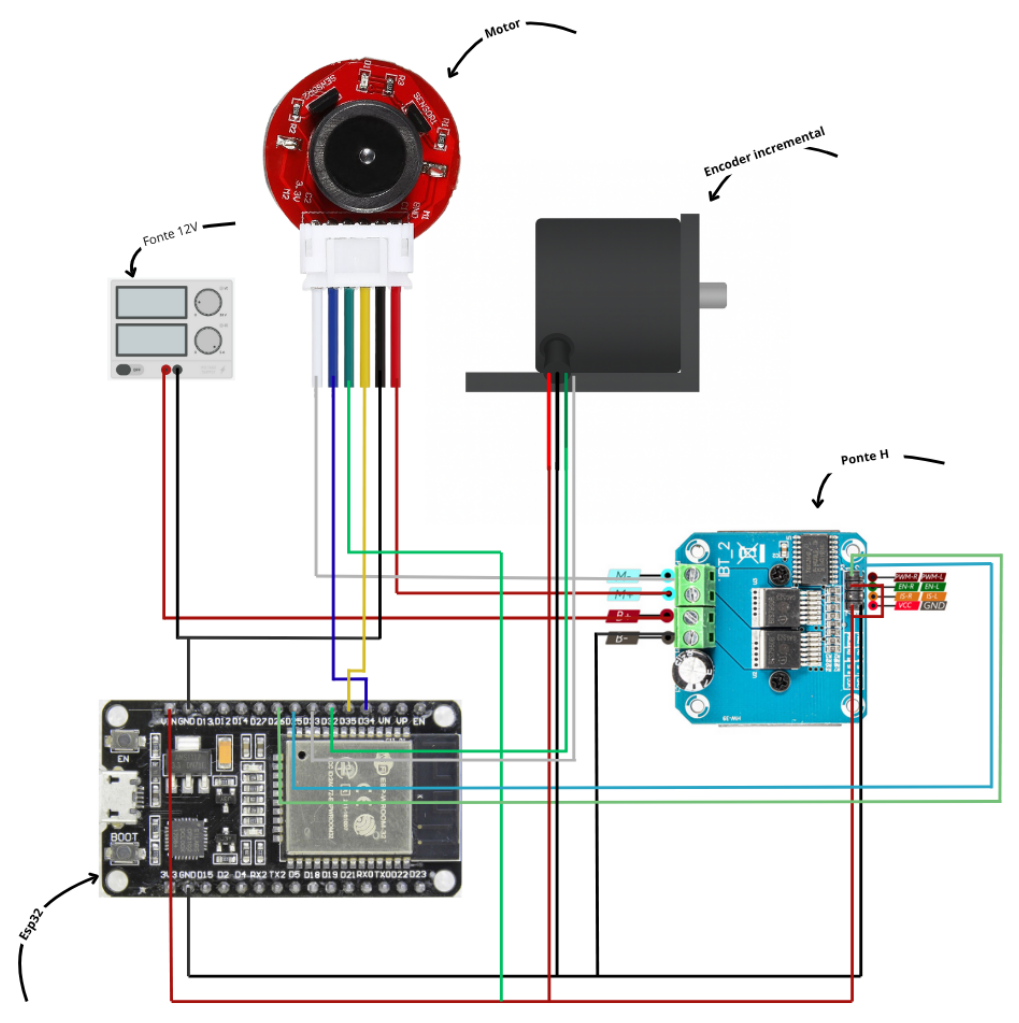
\includegraphics[width=0.9\columnwidth]{figures/circuito.png}
        \caption{Diagrama do circuito do pêndulo invertido rotacional com ESP32, BTS7960, motor DC com encoder Hall e encoder incremental do pêndulo.}
        \label{fig:circuito}
    \end{figure}


\subsection{Ambiente de Software}

    Para a simulação do sistema de controle do pêndulo invertido rotacional, será utilizado o ambiente de simulação \textbf{MATLAB/Simulink}. O Simulink permitirá a modelagem gráfica do sistema dinâmico e do controlador, além de possibilitar a simulação do comportamento do sistema em malha fechada. As equações diferenciais que governam o movimento do pêndulo serão implementadas no Simulink, e o controlador será testado em ambiente simulado antes de sua implementação em hardware.

    O MATLAB será utilizado para análise dos resultados, ajustes no controlador, e validação da solução por meio de simulações numéricas. Além disso, o MATLAB/Simulink facilita a integração com o Arduino, permitindo a comunicação entre a simulação e a implementação real do sistema.


\section{Cronograma de Execução}

    O cronograma detalhado para as etapas do projeto é apresentado na Tabela \ref{tab:cronograma}.

\begin{table}[H]
    \centering
    \caption{Cronograma de execução do projeto.}
    \label{tab:cronograma}
    \resizebox{\columnwidth}{!}{%
    \begin{tabular}{lll}
        \toprule
        \textbf{Etapa} & \textbf{Início} & \textbf{Fim} \\
        \midrule
        Etapa 1: Descrição do Problema e Revisão Teórica & 22/07/2025 & 01/08/2025 \\
        Etapa 2: Modelagem e Simulação & 02/08/2025 & 04/09/2025 \\
        Etapa 3: Projeto do Controlador & 05/09/2025 & 09/10/2025 \\
        Etapa 4: Implementação e Validação Experimental & 10/10/2025 & 12/11/2025 \\
        \bottomrule   
    \end{tabular}%
    }
\end{table}

\vspace{-6mm} % reduz espaço vertical entre as tabelas

\begin{table}[H]
    \centering
    \caption{Cronograma de execução da Etapa 1}
    \label{tab:cronograma-etapa1}
    \resizebox{\columnwidth}{!}{%
    \begin{tabular}{lll}
        \toprule
        \textbf{Tarefa} & \textbf{Início} & \textbf{Fim} \\
        \midrule
        Definição do Problema & 22/07/2025 & 24/07/2025 \\
        Revisão Bibliográfica & 25/07/2025 & 27/07/2025 \\
        Levantamento de Materiais e Métodos & 28/07/2025 & 30/07/2025 \\  
        Detalhes Finais e Apresentação & 31/07/2025 & 01/08/2025 \\
        \bottomrule   
    \end{tabular}%
    }
\end{table}

\vspace{-6mm}

\begin{table}[H]
    \centering
    \caption{Cronograma de execução da Etapa 2}
    \label{tab:cronograma-etapa2}
    \resizebox{\columnwidth}{!}{%
    \begin{tabular}{lll}
        \toprule
        \textbf{Tarefa} & \textbf{Início} & \textbf{Fim} \\
        \midrule
        Modelagem Matemática & 02/08/2025 & 12/08/2025 \\
        Análise do Modelo & 13/08/2025 & 23/08/2025 \\
        Simulação Computacional & 24/08/2025 & 01/09/2025 \\
        Síntese dos resultados e Próximos passos & 02/09/2025 & 04/09/2025 \\
        \bottomrule   
    \end{tabular}%
    }
\end{table}

\vspace{-6mm}

\begin{table}[H]
    \centering
    \caption{Cronograma de execução da Etapa 3}
    \label{tab:cronograma-etapa3}
    \resizebox{\columnwidth}{!}{%
    \begin{tabular}{lll}
        \toprule
        \textbf{Tarefa} & \textbf{Início} & \textbf{Fim} \\
        \midrule
        Montagem do Protótipo & 05/09/2025 & 10/09/2025 \\
        Coleta de Dados Experimentais & 11/09/2025 & 21/09/2025 \\
        Comparação e Validação do Modelo & 22/09/2025 & 06/10/2025 \\
        Síntese dos Resultados e Próximos Passos & 07/10/2025 & 09/10/2025 \\
        \bottomrule   
    \end{tabular}%
    }
\end{table}

\vspace{-6mm}

\begin{table}[H]
    \centering
    \caption{Cronograma de execução da Etapa 4}
    \label{tab:cronograma-etapa4}
    \resizebox{\columnwidth}{!}{%
    \begin{tabular}{lll}
        \toprule
        \textbf{Tarefa} & \textbf{Início} & \textbf{Fim} \\
        \midrule
        Projeto do Controlador & 10/10/2025 & 20/10/2025 \\
        Simulação do Sistema Controlado & 21/10/2025 & 28/11/2025 \\
        Implementação e Testes no Protótipo & 29/11/2025 & 08/11/2025 \\
        Análise Crítica e Conclusão Final & 09/11/2025 & 12/11/2025 \\
        \bottomrule
    \end{tabular}%
    }
\end{table}

    % \begin{itemize}
    %     \item BREGANON, R. et al. Desenvolvimento de sistemas de pêndulos invertidos como ferramentas didáticas em cursos de engenharia de controle e automação. \textit{HOLOS}, v. 7, p. 1–14, 2021. DOI: 10.15628/holos.2021.10351.
    
    %     \item DUART, J. L. et al. Dynamic modeling and simulation of a rotational inverted pendulum. \textit{Journal of Physics: Conference Series}, v. 792, 2017.
    
    %     \item CASAS, V. M. et al. Construção e projeto de controle de um protótipo de pêndulo invertido rotacional. \textit{EasyChair Preprint}, 2024.
    
    %     \item JAKOBSSON, S. Á. Control of a rotary inverted pendulum system using computer vision. Master’s Thesis – Reykjavik University, 2024.
    
    %     \item YAMANE, L. de S. Projeto mecânico e síntese do controlador de um pêndulo de Furuta. Trabalho de Conclusão de Curso (Engenharia Mecânica) – Universidade Federal do Amazonas, 2020.
    % \end{itemize}


%----------------------------------------------------------
\nocite{yamane2021}
\printbibliography

%----------------------------------------------------------

\end{document}